\documentclass[11pt]{beamer}
\usetheme{Singapore}
\usepackage[utf8]{inputenc}
\usepackage[french]{babel}
\usepackage[T1]{fontenc}
\usepackage{amsmath}
\usepackage{amsfonts}
\usepackage{amssymb}
\author{Le groupe MkRpg}
\title{Présentation du projet MkRpg}
%\setbeamercovered{transparent} 
\setbeamertemplate{navigation symbols}{} 
\renewcommand{\insertnavigation}[1]{\hfill
\includegraphics[scale=.5]{main.png}~\vspace{-.2cm}}
% Raoul :
%\renewcommand{\insertnavigation}[1]{\hfill
\includegraphics[scale=.25]{raoul.png}~\vspace{-.2cm}}
%\setbeamertemplate{headline}{}
%\logo{} 
%\institute{} 
%\date{} 
%\subject{} 
\begin{document}

\begin{frame}
\titlepage
\end{frame}

\begin{frame}{Sommaire}
\tableofcontents
\end{frame}

%%%%%%%%%%%%%%%%%%%%%%%%%%%%%%%%%%%%%%%%%%%%%%%%%%%%%%%%%%%%%%%%%%%%%%



%%%%%%%%%%%%%%%%%%%%%%%%%%%%%%%%%%%%%%%%%%%%%%%%%%%%%%%%%%%%%%%%%%%%%%
\section{Client}
    \begin{frame}
        \frametitle{Sommaire}
        \tableofcontents[currentsection]
    \end{frame}

\subsection{Architecture}
\begin{frame}{Architecture}
	\begin{center}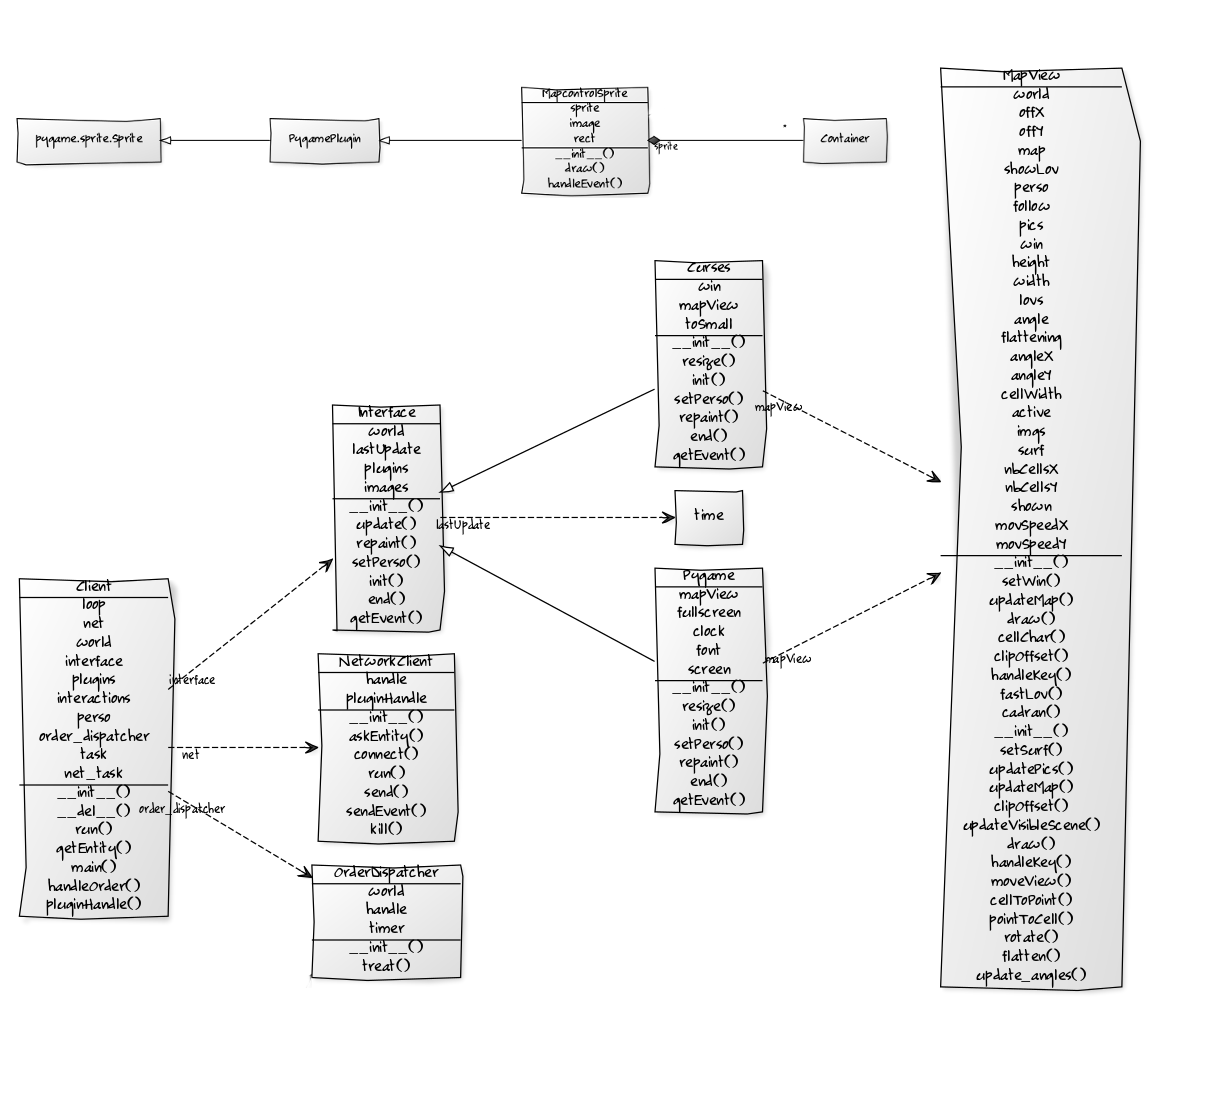
\includegraphics[scale=0.21]{uml_pygame.png}\end{center}
\end{frame}

\begin{frame}{Les bienfaits de l'asynchrone}
\begin{itemize}
\item utilisation du module \textbf{asyncio} et des nouveaux mots-clés async et await
\item pas de threads
\item robustesse
\item calculs dans d'autres processus
\item intégrable aux plugins
\end{itemize}
\end{frame}

\subsection{Interface pygame}
\begin{frame}{Interface pygame - features}
	\begin{itemize}
		\item mise en cache
    \item changement de cartes
    \item rotation de carte
    \item zoom/dezoom
    \item affichage d'objets
    \item système de gui
    \item plugins d'affichage
	\end{itemize}
\end{frame}

\begin{frame}{Interface pygame}
	\begin{itemize}
    \item performances : raisonnables, 30 FPS, quelques lags quand on affiche des parties trop importantes de la map
		\item[]
    \item stabilité : quelques exceptions non capturées (rotation de carte), sinon affichage très stable
	\end{itemize}
\end{frame}

\begin{frame}{Interface pygame}
	\begin{center}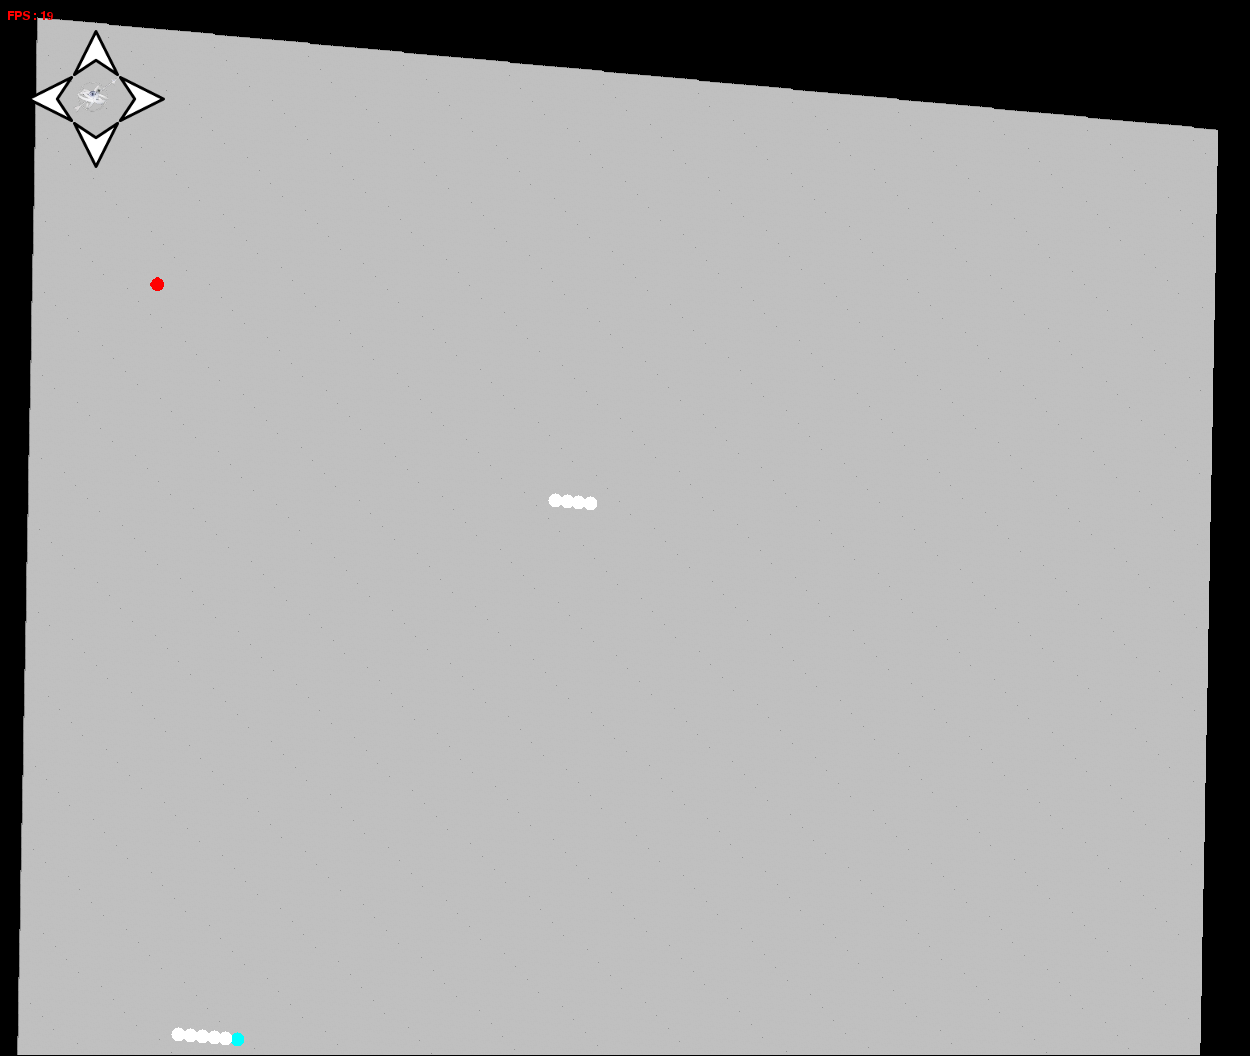
\includegraphics[scale=0.2]{game_screenshot.png}\end{center}
\end{frame}

\begin{frame}{Interface pygame - GUI}
	\begin{center}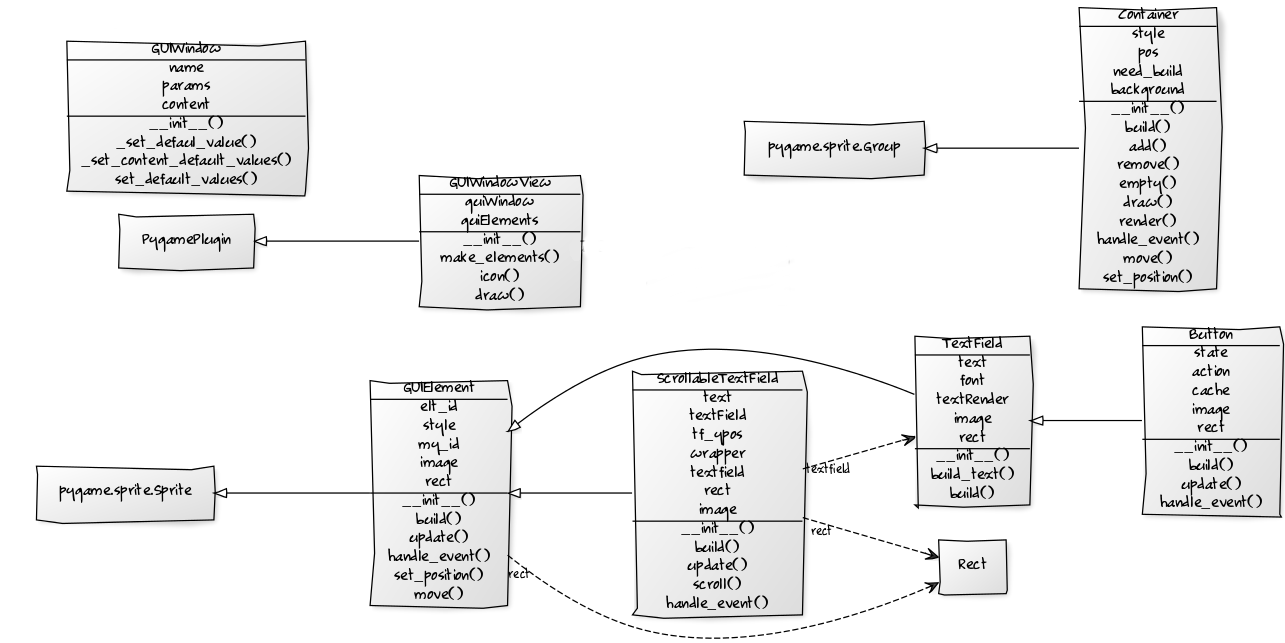
\includegraphics[scale=0.25]{gui_uml.png}\end{center}
\end{frame}

%%%%%%%%%%%%%%%%%%%%%%%%%%%%%%%%%%%%%%%%%%%%%%%%%%%%%%%%%%





\setbeamertemplate{navigation symbols}{} 
\renewcommand{\insertnavigation}[1]{\hfill
\includegraphics[scale=.5]{main.png}~\vspace{-.2cm}}
\section{Éditeur}

    \begin{frame}
        \frametitle{Contents}
        \tableofcontents[currentsection]
    \end{frame}

\subsection{Objectifs}
\begin{frame}{Objectifs}
	\begin{itemize}
	\item Création des jeux
		\item Modification de jeux (en cours de campagne)
		\item Création de XML pour le serveur et les clients
		\item Utilisation d'abstractions pour l'édition (Ajout de vie, déroulement du temps, ...)
	\end{itemize}
\end{frame}

\subsection{Choix techniques}
\begin{frame}{Outils utilisés}
	\textbf{Langage de programmation :}
	C++
	\begin{itemize}
		\item Sécurité et confort du typage
		\item Performances
		\item Lisibilité du code (.h)
	\end{itemize}
	
	~
	
	\textbf{Interface graphique :}
	Framework Qt
	\begin{itemize}
		\item Connaissances préalables
		\item Outils de création de fenêtre puissant (Qt Designer)
		\item API haut niveau (lecture/écriture XML)
	\end{itemize}
	
	~
	
	\textbf{Inconvénients :} Duplication de code
\end{frame}

\subsection{Architecture}
\begin{frame}{Architecture}
	\textbf{Architecture globale :}
	\begin{itemize}
		\item Modèle :
		\begin{itemize}
			\item Représentation interne des données
			\item Accesseurs et mutateurs pour assurer des invariants
		\end{itemize}
		\item Interface :
		\begin{itemize}
			\item Accès aux données
			\item Ajout et modification d'éléments
			\item Abstractions des mécanismes d'événements et d'actions
		\end{itemize}
	\end{itemize}

\end{frame}

\begin{frame}{Interface}
	\textbf{Architecture Qt classique}
	\begin{itemize}
		\item Sous classe pour les \textit{widgets} d'affichage spécifiques
		\item Utilisation de l'API Model/View
	\end{itemize}
	
	~
	
	\textbf{Patrons de conception utilisés}
	\begin{itemize}
		\item \textit{Fabrique} : Éditeurs spécifiques aux objets
		\item \textit{Singleton} : Options de l'éditeur (dossiers par défaut, ...)
	\end{itemize}
\end{frame}


\begin{frame}{Modèle}
	\textbf{Classe de base : } \texttt{GameObject} 
	\begin{itemize}
		\item Utilisation du polymorphisme (écriture de XML, édition)
		\item Organisation des jeux en arbre
		\item Éléments communs : 
		\begin{itemize}
			\item Paramètres
			\item Drapeaux
			\item Événements
			\item Ordres
		\end{itemize}
		\item Mécanismes d'information des modifications
		\item Facilité de libération de mémoire
		\item Identifiant unique
	\end{itemize}
\end{frame}

\begin{frame}{Modèle}
	\textbf{Héritage d'objet}
	\begin{itemize}
		\item Classe \texttt{InheritableObject}
		\item Distinction \texttt{Type/TypedObject}
		\item Redéfinition des valeurs des paramètres/drapeaux
	\end{itemize}
	
	~
	
	\textbf{Objets virtuels d'organisation :}
	\begin{itemize}
		\item \texttt{DefaultTypes}
		\item \texttt{GameObjectList}
		\item \texttt{GameObjectInventory}
	\end{itemize}
\end{frame}


\begin{frame}{Modèle}
	\textbf{Diagramme des classes}
	
	~
	
	\begin{center}
		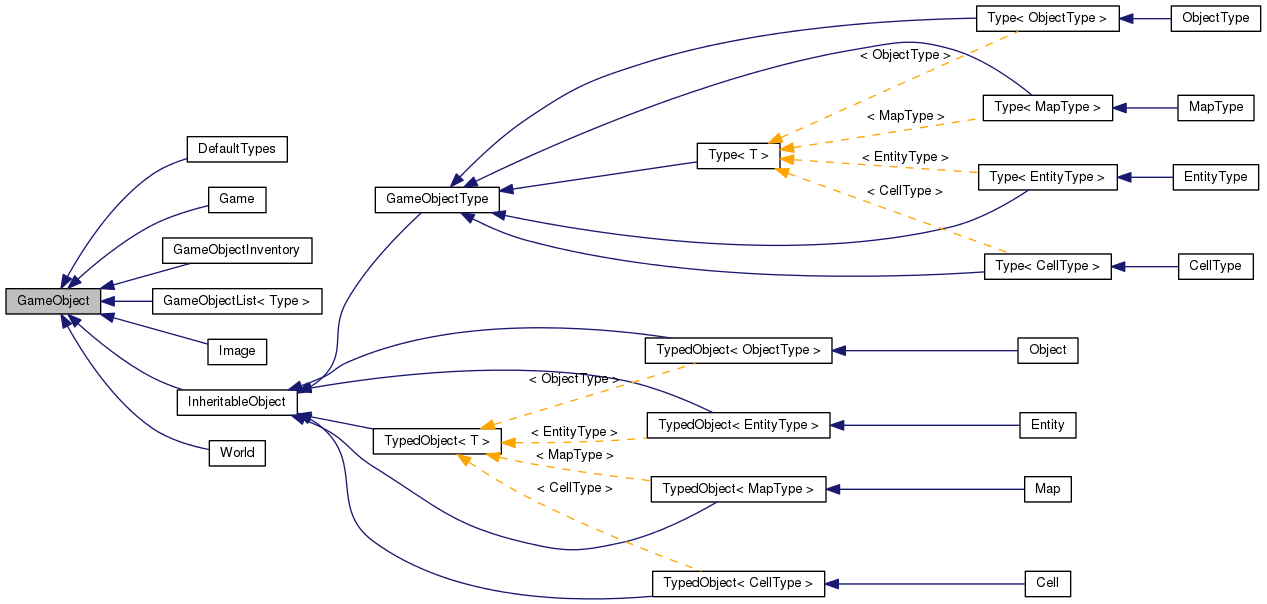
\includegraphics[scale=.24]{GameObject.png}
	\end{center}
\end{frame}


\begin{frame}{XML}
	\textbf{Export}
	\begin{itemize}
		\item XML du serveur : lisible par les serveur/clients
		\item XML de l'éditeur : contient des informations d'édition et d'organisation interne
	\end{itemize}
	
	~
	
	\textbf{Import}
	
	Import de jeux par lecture de XML (éditeur)
\end{frame}

\section{Software Engineering Tools}
 \begin{frame}
        \frametitle{Contents}
        \tableofcontents[currentsection]
    \end{frame}
\subsection{Introduction}

\begin{frame}
    \frametitle{\secname~: Different SWE tools}
    \begin{itemize}
        \item Git (via GitHub)
        \item Convention (pylint)
        \item Documentation (doxygen)
        \item Test (Travis, Unittest)
    \end{itemize}
\end{frame}

\subsection{Git}

\begin{frame}
    \frametitle{\secname~: Utilisation of Git}
    \begin{itemize}
        \item version control system (commits)
        \item different branches 
        \item decentralized
    \end{itemize}
\end{frame}

\begin{frame}
    \frametitle{\secname~: Utilisation of GitHub}
    Why ?
    \begin{itemize}
        \item simple to use
        \item issues
        \item compatible with continuous integration tools 
        \item nice graphs 
    \end{itemize}
\end{frame}

\begin{frame}
    \frametitle{\secname}
    \begin{itemize}
    	\item \textit{https://github.com/mkRPGDev/mkRPG}
        \item $16$ issues
        \item $\simeq 600$ commits
        \item $17$ branches whose one for documentation
    \end{itemize}
\end{frame}

\subsection{Convention}
\begin{frame}
    \frametitle{\secname~: \href{https://www.python.org/dev/peps/pep-0008/}{PEP 8 -- Style Guide for Python Code}}
    \begin{itemize}
        \item code lay-out
        \item whitespace in expressions and statements
        \item documentation strings
        \item naming conventions
    \end{itemize}
\end{frame}

\begin{frame}
    \frametitle{\secname~: Pylint - enforce coding standard}
    \begin{itemize}
        \item errors and warning
        \item statistics and note 
        \item different format
        \item pre-commit hook 
    \end{itemize}  
    Our code : $5.09/10$
\end{frame}

\subsection{Documentation}
\begin{frame}
    \frametitle{\secname~: Why ?}
    \begin{itemize}
        \item readable for the writer
        \item understandable by others 
        \item easy debug
    \end{itemize}
\end{frame}

\begin{frame}
    \frametitle{\secname~: Doxygen}
    Documentation generated by doxygen
    \begin{itemize}
    	\item automatically generated
        \item html or tex
        \item nice graphs
    \end{itemize}
\end{frame}

\begin{frame}
    \frametitle{\secname~: Doxygen}
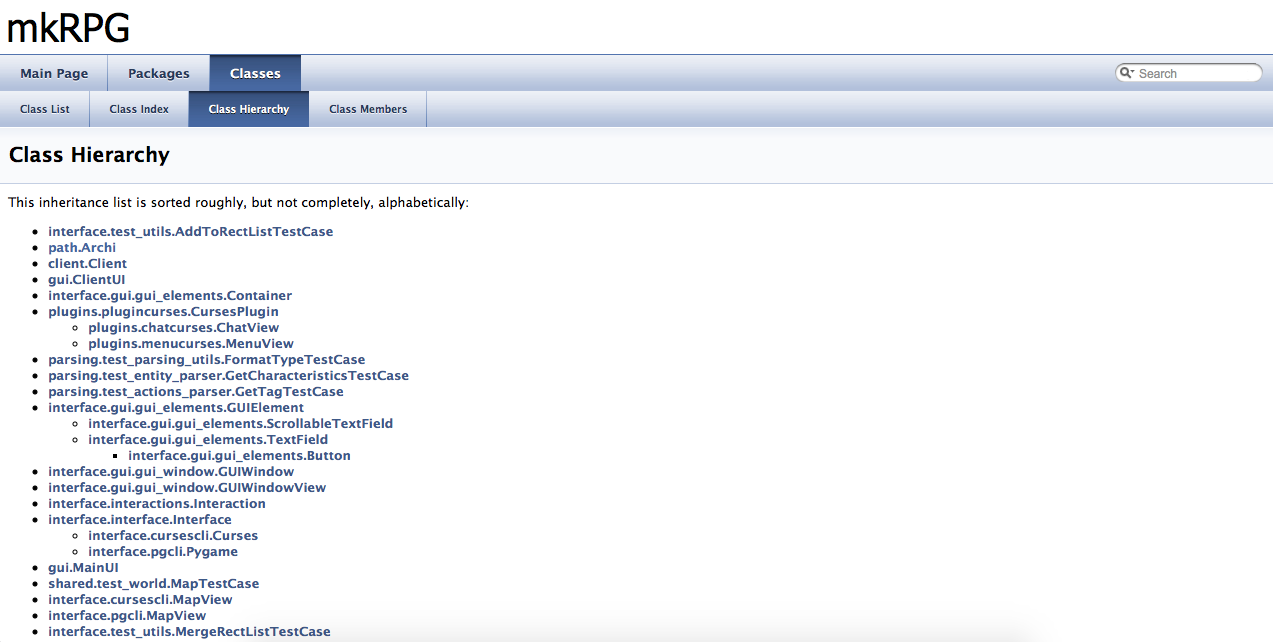
\includegraphics[scale=0.3]{doxygen}
\end{frame}

\subsection{Tests}
\begin{frame}
    \frametitle{\secname~}
    \begin{itemize}
    	\item \textit{"There ARE bugs in your code."}
        \item Static analysis (pylint)
        \item Unit testing (unittest)
    \end{itemize}
\end{frame}

\subsubsection{Unit testing}
\begin{frame}
    \frametitle{\secname~: Unittest}
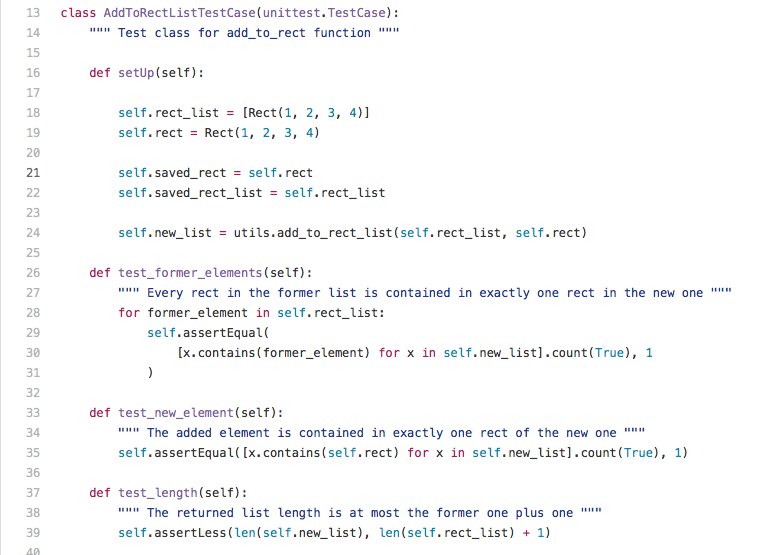
\includegraphics[scale=0.4]{unittest}
\end{frame}

\subsubsection{Continuons Integration}
\begin{frame}
    \frametitle{\secname~: Travis}
    Every modification of code runs code on server to check if anything bad happend
    \begin{itemize}
    	 \item Unittest (unit testing)
        \item Doxygen (documentation)
        \item Pylint (static code analysis)
    \end{itemize}
\end{frame}

\begin{frame}
    \frametitle{\secname~: Travis}
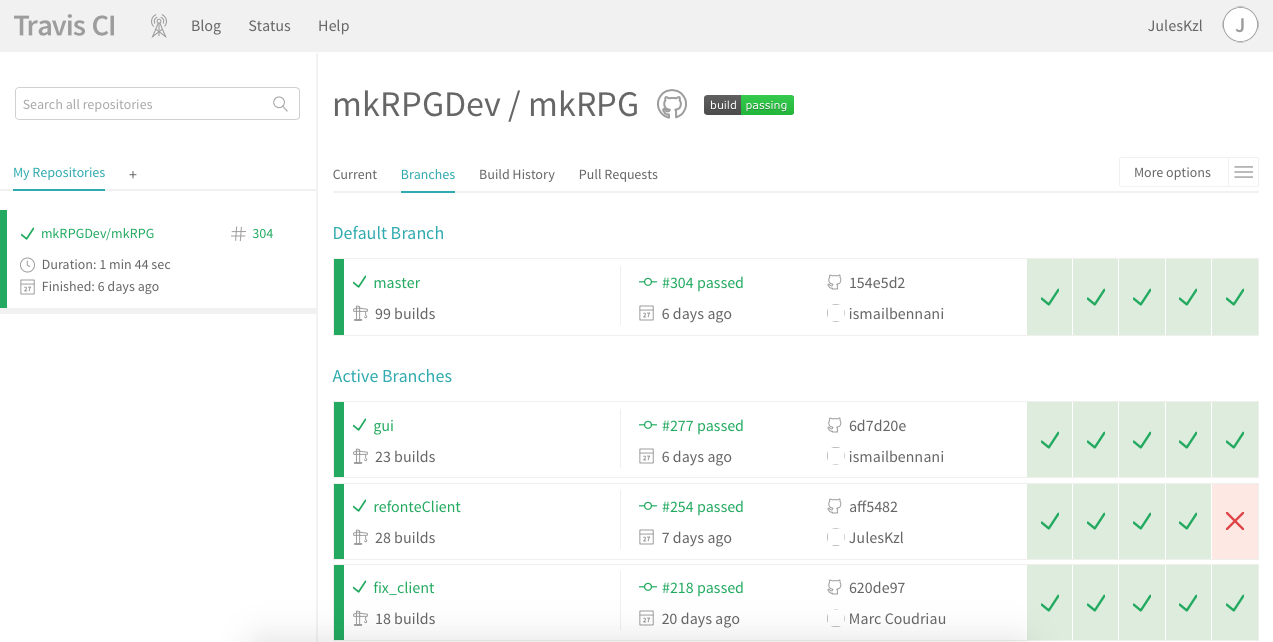
\includegraphics[scale=0.3]{travis}
\end{frame}


\section{Commentaires}

    \begin{frame}
        \frametitle{Contents}
        \tableofcontents[currentsection]
    \end{frame}
    
\begin{frame}{Difficultés - Choix discutables \textit{a posteriori}}
	\textbf{Pygame}
	\begin{itemize}
		\item efficace pour de petits projets
		\item pas adapté aux moyens/gros projets
		\item quelques problèmes de compatibilité
		\item manque de documentation avancée et/ou d'exemples d'utilisation avancés suffisamment commentés
	\end{itemize}
\end{frame}


\begin{frame}{Remarques}
	\textbf{Général}
	\begin{itemize}
		\item Préciser les architectures avant de coder
		\item Faire avancer les différents composants à la même vitesse
		\item On a sous-estimé la charge de travail liée à l'affichage
		\item[]
		\item Quelques problèmes de communication en cours de route
		\item Gros problème de partage des taches malgré quelques tentatives pour mieux les répartir
		\item[]
		\item Plus de tests nécessaires, code parfois difficile à tester
	\end{itemize}
\end{frame}


\begin{frame}{Perspectives}
	\textbf{Interface}
	\begin{itemize}
		\item Architecture de l'interface cohérente et pratique
		\item Système de plugin tout puissant (tout est modifiable à travers des plugins)
		\item Interface soutenable a moyen terme pour des jeux de taille moyenne
	\end{itemize}
	
	~
	
	\textbf{Éditeur}
	\begin{itemize}
		\item Définition d'un langage d'ordre
		\item Ajout d'abstractions dans l'éditeur
		\item Révisions du XML (pour que XML serveur $\subset$ XML éditeur)
	\end{itemize}
\end{frame}


\end{document}
